\section{Linear Algebra Approach}
\subsection{Basic Concepts}
A formal mathematical description of quantum mechanics is essentially linear algebra in a Hilbert space.
The "state" of quantum particle is represented by a vector $\ket{\psi} \in \hilbert$: a Hilbert space.
\dfn{Observable, Hermitian Operator}{
  A physical quantity(\emph{observable}) $A$ is represented by a Hermitian (self-adjoint) operator $\hat{A}$ acting on the state vector $\ket{\psi}$:
  \begin{align}
    \hat{A} & = \hat{A}^\dagger, \quad \hat{A} \ket{a} = a \ket{a}, \quad a \in \real
  \end{align}
  where $\hat{A}^\dagger$ is \emph{Hermitian conjugate} of $\hat{A}$, and $\ket{a}$ is an \emph{eigenstate} of the operator $\hat{A}$ with eigenvalue $a$.
}
and we postulate that the probability of finding the system in the state $\ket{\phi}$ from another state $\ket{\psi}$ is given by the inner product:
\prcp{Born's Probability Interpretation}{
  The probability of finding the system in the state $\ket{\phi}$ from another state $\ket{\psi}$ is given by:
  \begin{align}
    P(\phi | \psi) & = |\braket{\phi}{\psi}|^2
  \end{align}
  where $\braket{\phi}{\psi}$ is the inner product of the two state vectors.
}

\begin{wrapfigure}[6]{r}[0pt]{0.5\textwidth}
  \centering
  \vspace*{-0.8cm}
  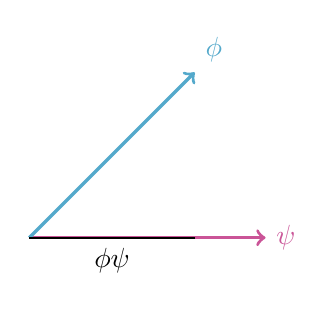
\begin{tikzpicture}[scale=1.5]
    \draw[very thick, magenta!60!gray, ->] (0,0) -- (2,0) node[right] {$\ket{\psi}$};
    \draw[very thick, cyan!60!gray,    ->] (0,0) -- (1.4,1.4) node[above right] {$\ket{\phi}$};
    \draw[thick] (0,0) -- (1.4, 0) node[midway, below] {$\braket{\phi}{\psi}$};
  \end{tikzpicture}
  \vspace*{-0.5cm}
  \caption{Inner product in a Hilbert space}
  \label{fig:inner_product}
\end{wrapfigure}
Intuitively, the inner product $\braket{\phi}{\psi}$ indicates how "close" the two states $\ket{\phi}$ and $\ket{\psi}$ are:
Note that the inner product is a complex number, and the probability is given by the square of the absolute value of the inner product.



\subsection{Position and Momentum in Quantum Mechanics}
The position and momentum of a particle are represented by operators $\hat{x}$ and $\hat{p}$, and we impose the canonical commutation relation onto these operators:
\prcp{Canonical commutation relation}{
  The position and momentum operators satisfy the following commutation relation:
  \begin{align}
    \commt{\hat{x}_i}{\hat{p}_j} & = i \hbar \delta_{ij}
  \end{align}
  where $\hbar$ is the reduced Planck's constant.
}
This implies that in the position basis, the momentum operator acts as a derivative operator (refer to Principle \ref{prcp:canonical-commutation-relation}):
\begin{align}
  \hat{p} \ket{x} & = -i \hbar \pdv{}{x} \ket{x}
\end{align}

The eigenstates of $\hat{x}$ and $\hat{p}$ are denoted as $\ket{x}$ and $\ket{p}$, respectively, and they satisfy the completeness relation:
\prcp{Completeness relation of Continuous Eigenbasis}{
  for $\ket{x}$ and $\ket{p}$, the following completeness relation holds:
  \begin{alignat}{2}
    \braket{x}{x'}                            & = \delta(x - x'), & \quad \braket{p}{p'}                 & = \delta(p - p') \\
    \iff \quad \int \odif{x} \, \ketbra{x}{x} & = \idty,          & \quad \int \odif{p} \, \ketbra{p}{p} & = \idty
  \end{alignat}
}
Now, we can define the position and momentum wavefunctions $\psi(x), \psi(p)$, whose magnitude squared gives the probability density of finding the particle at a certain position $x$ or momentum $p$:
\dfn{Wavefunction}{
  The \emph{wavefunction} $\psi(x)$ of a quantum particle is defined as the inner product of the state vector $\ket{\psi}$ with the position eigenstate $\ket{x}$:
  \begin{align}
    \psi(x) & = \braket{x}{\psi}
  \end{align}
  Colloquially, wavefuntion represents the probability amplitude of finding the particle at position $x$ in state $\ket{\psi}$.
}
\nt{
  We can equally define a wavefunction in the momentum basis:
  \begin{align}
    \psi(p) & = \braket{p}{\psi}
  \end{align}
  in which the $\hat{x}$ operator becomes a derivative operator w.r.t. $p$:
  \begin{align}
    \hat{x} \ket{p} & = i \hbar \pdv{}{p} \ket{p}
  \end{align}
}

\subsection{Unitary Transformations: Shift Operator and Fourier Transform}
Now, consider a shift operator $\hat{S}(a)$ that shifts the position eigenstate $\ket{x}$ by a constant $a$:
\dfn{Shift Operator}{
  The \emph{shift operator} $\hat{S}(a)$ is defined as:
  \begin{align}
    \hat{S}(a) \ket{x} & = \ket{x + a}
  \end{align}
}
From the discussion in Sec. \ref{sec:dual-der},
\thm{Commutator of Shift Operator}{
  For operators satisfying the commutation relation $\commt{\hat{D}}{\hat{x}} = 1$,
  \begin{align}
    \commt{\hat{S}(a)}{x} & = a \hat{S}(a) \implies \hat{S}(a) = e^{a D}
  \end{align}
}
since $\hat{p} = -i \hbar \hat{D} \iff \hat{D} = \frac{\hat{p}}{-i \hbar}$, we can write the shift operator as:
\begin{align}
  \hat{S}(a) & = e^{\frac{a \hat{p}}{-i \hbar}} = e^{i \frac{\hat{p}}{\hbar} a}
\end{align}


\dfn{Fourier Transform in Quantum Mechanics}{
  The position wavefunction $\braket{x}{\psi}$ can be expanded in the momentum basis $\ket{p}$, by the \emph{Fourier transform}:
  \begin{align}
    \braket{x}{\psi} & = \int \odif{p} \, \braket{x}{p} \braket{p}{\psi} = \int \frac{\odif{p}}{\sqrt{2 \pi \hbar}} e^{i \frac{p}{\hbar} x} \braket{p}{\psi}
  \end{align}
}

\section{Harmonic Oscillator}